\documentclass[assignment = 4]{homework}

\usepackage{caption, subcaption, pdfpages, float}
\usepackage{graphics, wrapfig, pgf, graphicx}
\usepackage{enumitem}
\graphicspath{{../resultados/}}


% pacotes para importar código
\usepackage{caption, booktabs}
\usepackage[section, newfloat]{minted}
\definecolor{sepia}{RGB}{252,246,226}
\setminted{
    bgcolor = sepia,
    style   = pastie,
    frame   = leftline,
    autogobble,
    samepage,
    python3,
}
\setmintedinline{
    bgcolor={}
}

% ambientes de códigos de Python
\newmintedfile[pyinclude]{python3}{}
\newmintinline[pyline]{python3}{}
\newcommand{\pyref}[2]{\href{#1}{\texttt{#2}}}

% \SetupFloatingEnvironment{listing}{name=Código}
% \captionsetup[listing]{position=below,skip=-1pt}

\usepackage{csquotes}
\usepackage[style=verbose-ibid,autocite=footnote,notetype=foot+end,backend=biber]{biblatex}
\addbibresource{referencias.bib}
\usepackage[section]{placeins}

\usepackage[hidelinks]{hyperref}
\usepackage[noabbrev, nameinlink, brazilian]{cleveref}
\hypersetup{
    pdftitle  = {MC920 - Trabalho 4 - 187679},
    pdfauthor = {Tiago de Paula}
}

\newcommand{\textref}[2]{
    \hyperref[#2]{#1 \ref*{#2}}
}

\usepackage{import, multirow}
\usepackage{tikz}
\usetikzlibrary{matrix}
\usetikzlibrary{positioning}

\newenvironment{kmatrix}[1][1.3cm]{
    \begin{tikzpicture}[node distance=0cm]
        \tikzset{square matrix/.style={
                matrix of nodes,
                column sep=-\pgflinewidth, row sep=-\pgflinewidth,
                nodes={draw,
                    minimum height=#1,
                    anchor=center,
                    text width=#1,
                    align=center,
                    inner sep=0pt
                },
            },
            square matrix/.default=#1
        }
}{
    \end{tikzpicture}%
}

\newcommand*{\Scale}[2][4]{\scalebox{#1}{\ensuremath{#2}}}%

\newcommand{\red}[1]{\textcolor{red}{\textbf{#1}}}

% \date{1 de dezembro de 2020}

\begin{document}

    \pagestyle{main}

    \section{Introdução}
% TODO: reescrever texto
% TODO(?): imagens
% TODO(?): REF merriam-webster

Esteganografia é uma técnica de comunição secreta, onde a mensagem é escondida em parte de outro texto ou objeto. Dessa forma, apenas o remetente e o destinatário saberiam onde encontrar a mensagem \red{encoberta}, podendo se comunicar em sigilo.

% TODO(?): Social steganography

Isso é diferente da criptografia em que a mensagem continua visível, mas sem sentido algum, exceto para os comunicadores, que conseguem descriptografar a mensagem. Normalmente, a criptografia acaba sendo aplicada na esteganografia, para garantir maior segurança no processo.

Nesse trabalho, foram implementados algoritmos simples de esteganografia em imagens digitais, com objetivo de analisar os casos de uso e os limites desse processo. Além disso, foram discutidos alguns traços comuns deixados na esteganografia e possíveis soluções para esses problemas.


    \section{O Programa}

Neste trabalho foram desenvolvidas duas ferramentas, \texttt{codificar.py} e \texttt{decodificar.py} que fazem todo o processo de esteganografia. Boa parte do código delas é compartilhado pelos arquivos na pasta \texttt{lib} do código-fonte. Além disso, também existem duas ferramentas usadas para análise dos resultados, a \texttt{dist.py} e \texttt{plano.py}, que não são necessárias para a execução do \red{processo de esteganografia}.

Todas as ferramentas foram desenvolvidas e \red{testadas} em Python 3.6 ou superior. Além da biblioteca padrão da linguagem, foram utilizados também os pacotes OpenCV, para entrada e saída de imagens, e Numpy \red{1.17}, para aplicação vetorizada da esteganografia.

\subsection{Código-Fonte}

    \begin{description}
        \item[codificar.py] Pacote interno com as operações de limiarização.

        \item[decodificar.py] Pacote interno com as operações de limiarização.

        \item[lib] Pacote interno com as operações de limiarização.

        \begin{description}
            \item[bits.py] Wrapper para a chamada das funções em C.

            \item[estego.py] Funções de cálculo do limiar da vizinhança do pixel.

            \item[permuta.py] Operações de mínimo, máximo, média, desvio padrão e mediana.

            \item[args.py] Tratamento de entrada e saída do programa.

            \item[inout.py] Tratamento de entrada e saída do programa.

            \item[tipos.py] Tipos para checagem estática com MyPy.
        \end{description}

        \item[plano.py] Pacote interno com as operações de limiarização.

        \item[dist.py] Pacote interno com as operações de limiarização.
    \end{description}


    \section{Implementação} \label{sec:implementacao}

O primeiro passo no algoritmo de codificação implementado da esteganografia foi transformar o dados do arquivo de entrada em um vetor de bits. Assim, a mensagem ``IC'', dada pelos bytes 0x49 e 0x43, seria representada pelo vetor $[1, 0, 0, 1, 0, 0, 1, 0, 1, 1, 0, 0, 0, 0, 1, 0]$. Para que seja possível a recuperação, também é adicionado um vetor de 64 bits antes do vetor de bits da imagem, representando o tamanho desse vetor.

Para injetar esse vetor na imagem são feitas algumas manipulações binárias simples. Para cada byte da imagem é aplicada uma máscara responsável por zerar o plano de bit especificado. Após isso, o bit que será inserido é deslocado (por \textit{bitshift}) para a posição certa e aplicado por um \textit{bitwise or} no byte da imagem novamente. Isso é feito até encerrar o vetor de bits

No código-fonte entregue, o mesmo processo é feito de forma vetorizada, utilizando uma matriz booleana para indexação.

Para a decodificação o processo é ainda mais simples. Basta extrair o plano de bit correto em um vetor de bits, recuperar o tamanho do arquivo nos primeiros 64 bits e usar isso para recuperar o vetor dos bits que realmente fazem parte do arquivo. O resultado é uma mera aglutinação desses bits em caracteres ou bytes.

\subsection{Permutação} \label{sec:permutacao}

O modelo anterior insere os bits sempre do começo pro final da imagem, o que pode gerar marcas bem claras na imagem \red{(resultados\qm)}. Uma maneira de evitar isso é distribuindo os dados do arquivo por toda a imagem, como é feito na ferramenta com a opção \mintinline{bash}{--permuta} ou \mintinline{bash}{-p}.

Nesse método basicamente é feita uma permutação da matriz booleana de indexação, inserindo os dados em posições mais distribuídas \red{pela} imagem. Para evitar o surgimento de algum padrão de bits, os dados da imagem também são permutados antes da inserção.

De forma a tornar o método reversível, mas imprevisível, em cada execução é gerada uma chave aleatória. Essa chave é usada como semente para o gerador pseudo-aleatório, sendo depois inserida nos últimos 64 bits do plano especificado na imagem. Todo esse método de permutação funciona apenas com a versão 1.17 ou superior de Numpy.

Com o tamanho fixado nos primeiros 64 bits e a chave nos últimos 64 bits, os dados dispersos na imagem podem ser facilmente recuperados, revertendo o processo anterior. Para indicar se houve a permutação na esteganografia ou não, a ferramenta usa o primeiro bit do plano de bits, efetivamente reduzindo o tamanho representável para 63 bits. Assim, a ferramenta de decodificação consegue recuperar os dois métodos, sem necessidade de indicação do usuário.


    \section{Resultados}

%% TODO %%
%
% Geral
% x Assinatura [mon]
% x Texto Pequeno [mon][wat]
% - Texto Grande [bab|pep]
% - Binario (Imagem / Zip) [bab|pep]
%
% Permutado
% - Texto Pequeno [mon] -- Tamanho + Chave
% - Texto Grande [bab|pep]
% - ?: Binário
%
% Plano de bit
% - 0, 1, 2
% - ?: 3, 5, 7

\subsection{Técnica Padrão}

\subsubsection{Assinatura}

    Podemos ver pela \cref{fig:assinatura} que assinatura digitais, normalmente com menos de caracteres, são imperceptíveis na imagem como um todo. No plano de bit específico, a diferença também não é visível ao olho humano.

    O resultado na \cref{fig:assinatura:imagem} contém o texto ``Realizzato da Leonardo da Vinci™'', representado em UTF-8 por 35 bytes. Juntamente com o cabeçalho de 8 bytes, a assinatura ocupa 344 bits do plano menos significativo. Isso não chega a metade da primeira linha ($256 \times 3$ bits de capacidade).

    A imagem pode ser produzida por:

    \begin{minted}{bash}
        $ echo Realizzato da Leonardo da Vinci™ | python3 codificar.py imagens/monalisa.png -o saida.png
    \end{minted}

    E verficada com:

    \begin{minted}{bash}
        $ python3 decodificar.py saida.png
        Realizzato da Leonardo da Vinci™
        $ # OU
        $ python3 decodificar.py saida.png | diff -qs - <(echo Realizzato da Leonardo da Vinci™)
        Files - and /proc/self/fd/12 are identical
    \end{minted}

    \begin{figure}[H]
    \centering
    \begin{subfigure}{0.5\textwidth}
        \centering
        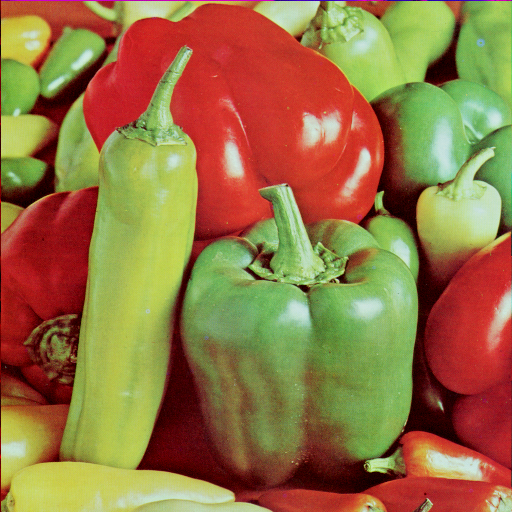
\includegraphics[width=0.85\textwidth]{mona_assin/imagem.png}
        \caption{Imagem com mensagem oculta.}
        \label{fig:assinatura:imagem}
    \end{subfigure}%
    \begin{subfigure}{0.5\textwidth}
        \centering
        \includegraphics[width=0.85\textwidth]{mona_assin/plano0.png}
        \caption{Plano 0.}
        \label{fig:assinatura:plano}
    \end{subfigure}\\[8pt]
    \begin{subfigure}{0.33\textwidth}
        \centering
        \includegraphics[width=0.85\textwidth]{mona_assin/pl0chb.png}
        \caption{Plano 0, canal azul.}
        \label{fig:assinatura:blue}
    \end{subfigure}%
    \begin{subfigure}{0.33\textwidth}
        \centering
        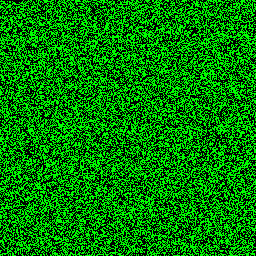
\includegraphics[width=0.85\textwidth]{mona_assin/pl0chg.png}
        \caption{Plano 0, canal verde.}
        \label{fig:assinatura:green}
    \end{subfigure}%
    \begin{subfigure}{0.33\textwidth}
        \centering
        \includegraphics[width=0.85\textwidth]{mona_assin/pl0chr.png}
        \caption{Plano 0, canal vermelho.}
        \label{fig:assinatura:red}
    \end{subfigure}%

    \caption{\texttt{monalisa.png} com uma assinatura de 35 bytes.}
    \label{fig:assinatura}
\end{figure}


    \section{Conclusão}

\end{document}
